% Options for packages loaded elsewhere
\PassOptionsToPackage{unicode}{hyperref}
\PassOptionsToPackage{hyphens}{url}
%
\documentclass[
]{article}
\usepackage{amsmath,amssymb}
\usepackage{iftex}
\ifPDFTeX
  \usepackage[T1]{fontenc}
  \usepackage[utf8]{inputenc}
  \usepackage{textcomp} % provide euro and other symbols
\else % if luatex or xetex
  \usepackage{unicode-math} % this also loads fontspec
  \defaultfontfeatures{Scale=MatchLowercase}
  \defaultfontfeatures[\rmfamily]{Ligatures=TeX,Scale=1}
\fi
\usepackage{lmodern}
\ifPDFTeX\else
  % xetex/luatex font selection
\fi
% Use upquote if available, for straight quotes in verbatim environments
\IfFileExists{upquote.sty}{\usepackage{upquote}}{}
\IfFileExists{microtype.sty}{% use microtype if available
  \usepackage[]{microtype}
  \UseMicrotypeSet[protrusion]{basicmath} % disable protrusion for tt fonts
}{}
\makeatletter
\@ifundefined{KOMAClassName}{% if non-KOMA class
  \IfFileExists{parskip.sty}{%
    \usepackage{parskip}
  }{% else
    \setlength{\parindent}{0pt}
    \setlength{\parskip}{6pt plus 2pt minus 1pt}}
}{% if KOMA class
  \KOMAoptions{parskip=half}}
\makeatother
\usepackage{xcolor}
\usepackage[margin=1in]{geometry}
\usepackage{longtable,booktabs,array}
\usepackage{calc} % for calculating minipage widths
% Correct order of tables after \paragraph or \subparagraph
\usepackage{etoolbox}
\makeatletter
\patchcmd\longtable{\par}{\if@noskipsec\mbox{}\fi\par}{}{}
\makeatother
% Allow footnotes in longtable head/foot
\IfFileExists{footnotehyper.sty}{\usepackage{footnotehyper}}{\usepackage{footnote}}
\makesavenoteenv{longtable}
\usepackage{graphicx}
\makeatletter
\def\maxwidth{\ifdim\Gin@nat@width>\linewidth\linewidth\else\Gin@nat@width\fi}
\def\maxheight{\ifdim\Gin@nat@height>\textheight\textheight\else\Gin@nat@height\fi}
\makeatother
% Scale images if necessary, so that they will not overflow the page
% margins by default, and it is still possible to overwrite the defaults
% using explicit options in \includegraphics[width, height, ...]{}
\setkeys{Gin}{width=\maxwidth,height=\maxheight,keepaspectratio}
% Set default figure placement to htbp
\makeatletter
\def\fps@figure{htbp}
\makeatother
\setlength{\emergencystretch}{3em} % prevent overfull lines
\providecommand{\tightlist}{%
  \setlength{\itemsep}{0pt}\setlength{\parskip}{0pt}}
\setcounter{secnumdepth}{5}
% definitions for citeproc citations
\NewDocumentCommand\citeproctext{}{}
\NewDocumentCommand\citeproc{mm}{%
  \begingroup\def\citeproctext{#2}\cite{#1}\endgroup}
\makeatletter
 % allow citations to break across lines
 \let\@cite@ofmt\@firstofone
 % avoid brackets around text for \cite:
 \def\@biblabel#1{}
 \def\@cite#1#2{{#1\if@tempswa , #2\fi}}
\makeatother
\newlength{\cslhangindent}
\setlength{\cslhangindent}{1.5em}
\newlength{\csllabelwidth}
\setlength{\csllabelwidth}{3em}
\newenvironment{CSLReferences}[2] % #1 hanging-indent, #2 entry-spacing
 {\begin{list}{}{%
  \setlength{\itemindent}{0pt}
  \setlength{\leftmargin}{0pt}
  \setlength{\parsep}{0pt}
  % turn on hanging indent if param 1 is 1
  \ifodd #1
   \setlength{\leftmargin}{\cslhangindent}
   \setlength{\itemindent}{-1\cslhangindent}
  \fi
  % set entry spacing
  \setlength{\itemsep}{#2\baselineskip}}}
 {\end{list}}
\usepackage{calc}
\newcommand{\CSLBlock}[1]{\hfill\break\parbox[t]{\linewidth}{\strut\ignorespaces#1\strut}}
\newcommand{\CSLLeftMargin}[1]{\parbox[t]{\csllabelwidth}{\strut#1\strut}}
\newcommand{\CSLRightInline}[1]{\parbox[t]{\linewidth - \csllabelwidth}{\strut#1\strut}}
\newcommand{\CSLIndent}[1]{\hspace{\cslhangindent}#1}
\usepackage{amsmath}
\usepackage{booktabs}
\usepackage{longtable}
\usepackage{array}
\usepackage{multirow}
\usepackage{wrapfig}
\usepackage{float}
\usepackage{colortbl}
\usepackage{pdflscape}
\usepackage{tabu}
\usepackage{threeparttable}
\usepackage{threeparttablex}
\usepackage[normalem]{ulem}
\usepackage{makecell}
\usepackage{xcolor}
\ifLuaTeX
  \usepackage{selnolig}  % disable illegal ligatures
\fi
\usepackage{bookmark}
\IfFileExists{xurl.sty}{\usepackage{xurl}}{} % add URL line breaks if available
\urlstyle{same}
\hypersetup{
  pdftitle={Trump's Tweets on Market Volatility},
  pdfauthor={Marcos Constantinou, Ryan Fellarhi \& Jonas Bruno},
  hidelinks,
  pdfcreator={LaTeX via pandoc}}

\title{Trump's Tweets on Market Volatility}
\author{Marcos Constantinou, Ryan Fellarhi \& Jonas Bruno}
\date{25.05.2025}

\begin{document}
\maketitle
\begin{abstract}
In this short paper, we aim to asses to what extent financial markets may react to Donald Trump's social media posts, and specifically the effect on average realised volatility. We do so using both ARMA-X and VAR models, with data spanning the 1st of January 2014, to the 7th of May 2025, over various time horizons and independent variables. We find limited evidence that there is a significant positive effect, and provide some explanations as to why this could be the case.
\end{abstract}

{
\setcounter{tocdepth}{2}
\tableofcontents
}
\newpage

\section{Introduction}\label{introduction}

\subsection{Motivation}\label{motivation}

Over the past 15 years social media has become an important
communication tool for politicians. One of the pioneers of this novel
approach has been Donald Trump, the 45th and 47th President of the United
States. Since his ban on Twitter after the January 6th riots, his quantity of
social media posts has drastically increased\footnote{Includes both Posts and Reposts}.

The content of his posts can sometimes have announcements or teases of future
political decisions. Note the recent infamous ``THIS IS A GREAT TIME TO BUY!!! DJT''
post sent just an hour before lifting his reciprocal tariffs. It is then not
improbable that agents in financial markets might take this information into
account in their decision making. This question has been asked before in the
literature, focusing rather on his first term.

This brings us to our research question: Do Donald Trumps Posts impact market Volatility?

\begin{figure}
\centering
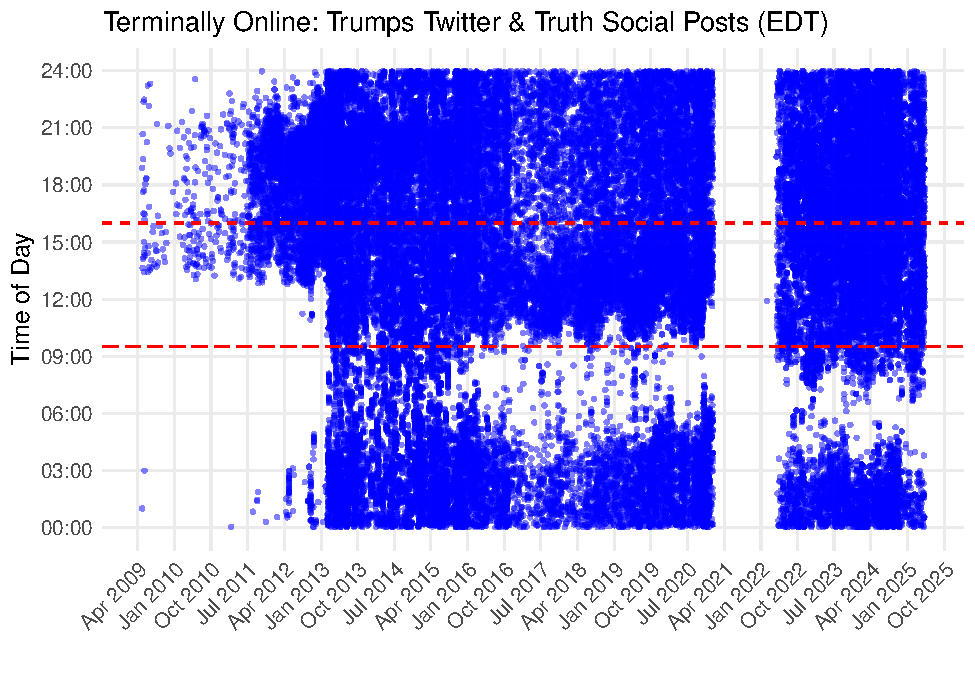
\includegraphics{trump_volatility_2025_files/figure-latex/fig1-1.pdf}
\caption{\label{fig:fig1}Terminally Online: Trump's Twitter \& Truth Social Posts (EDT)}
\end{figure}

\subsection{Literature Review}\label{literature-review}

Information is one of the most valuable assets in the financial market.
Its importance lies at the core of the ``Efficient Market Hypothesis'',
which states that the prices of assets fully reflect all
available information, adjusting immediately to any new data
Fama et al. (\citeproc{ref-famaAdjustmentStockPrices2003}{2003}) , and thereby creating a strong demand
for information flow. In addition, the ``Mixture of Distribution
Hypothesis'' states that the release of new information is closely linked
to movements in both realized and implied volatility
Andersen (\citeproc{ref-andersenReturnVolatilityTrading1996}{1996}), French \& Roll (\citeproc{ref-frenchStockReturnVariances1986}{1986}),
Vlastakis \& Markellos (\citeproc{ref-vlastakisInformationDemandStock2012}{2012}).

Consequently, a large part of the literature had focused on the relation
between announcements, news and market activity. For example,
Schumaker \& Chen (\citeproc{ref-schumakerTextualAnalysisStock2009}{2009}) use various linguistic and textual
representations derived from financial news to predict stock market
prices. Similarly, Ederington \& Lee (\citeproc{ref-ederingtonHowMarketsProcess1993}{1993}) analyze the impact
of macroeconomic news announcements on interest rate and foreign
exchange futures markets, particularly in terms of price changes and
volatility. Both studies, among others, find that prices--- such as stock
prices---react primarily within minutes after the release of new
information.

Recently, the world has witnessed the rise of the Internet
which revolutionized the dissemination and accessibility of information.
Social media enable investors, analysts or politicians to instantly
share their information, news or opinions. This led some studies to
focus on the communication dynamics of social platform to predict
changes in the returns of financial assets De Choudhury et al. (\citeproc{ref-dechoudhuryCanBlogCommunication2008}{2008}) \&
Bartov et al. (\citeproc{ref-bartovCanTwitterHelp2018}{2018}). In this context, the
impact of Trump's tweets on various financial and macroeconomic
variables has been analysed by several studies, especially during his
first mandate.

Using high-frequency financial data,
Gjerstad et al. (\citeproc{ref-gjerstadPresidentTrumpsTweets2021}{2021}) found an increase in uncertainty and
trading volume, along with a decline in the U.S. stock market---regardless
of the tweet's content. However, the effect was stronger when Trump used
confrontational words such as ``tariff'' or ``trade war.'' Some of his
announcements also influenced the U.S. dollar exchange rate Vlastakis \& Markellos (\citeproc{ref-vlastakisInformationDemandStock2012}{2012})
and certain market indices within minutes of the tweet being posted
Colonescu (\citeproc{ref-colonescuEffectsDonaldTrumps2018}{2018}) \& Kinyua et al. (\citeproc{ref-kinyuaAnalysisImpactPresident2021}{2021}).

Other scholars have shown that negative Trump tweets about specific
companies tended to reduce demand for their stocks Brans \& Scholtens (\citeproc{ref-bransHisThumbEffect2020}{2020}) \&
Mendels (\citeproc{ref-mendelsStanfordResearchSeries2019}{2019}), whereas some
other have shown that they also impact market volatility indices such as
the VIX Fendel et al. (\citeproc{ref-fendelPoliticalNewsStock2019}{2019}) or the Volfele Klaus \& Koser (\citeproc{ref-klausMeasuringTrumpVolfefe2021}{2021}).
The effects of his tweets also extended beyond the U.S.. For example,
Nishimura \& Sun (\citeproc{ref-nishimuraImpactsDonaldTrumps2025}{2025}) shows a
positive relationship between volatility in European stock markets and
tweeter activity of Trump, and this effect tends to intensify as public
intention for his tweet grows Nishimura \& Sun (\citeproc{ref-nishimuraImpactsDonaldTrumps2025}{2025}).

\section{Data}\label{data}

\subsection{Financial Data}\label{financial-data}

For our financial data, we decided to try to find minute-by-minute prices for
broad market indices. While the actual indices do not update their prices so often,
we had to take proxies under the form of ETF's that track them. Our 3 markets of
analysis are: SPY to track the S\&P500, VGK to track the FTSE Developed Europe
All Cap Index, and finally ASHR to track the CSI 300 China. We accessed this data
through a free stock API, Alpha Vantage. Our timeframe is from the first
of January 2014 to the 7th of May 2025.

We then had to transform this data to get our main variable of interest, Average
Hourly Volatility (AHV). Note that this is realised market volatility. We did so
with the following formula:
\[
\begin{aligned}
  v_t = \frac{1}{N}&\sum_{i=1}^N(\Delta p_{t,i})^2 
\end{aligned}
\]
Where \(\Delta p_t\) is the difference in price (open - close) and \(i\) represents
every minute.

We used a custom function in order to get the AHV for each open market hour. Note
that the first hour is from 9:30 am to 10:00 am since the market opens on a half-hour
but closes at 4:00 pm.

We can clearly see that the last few months show a new era of never seen before
levels of volatility. Shocks on volatility recently have reached, and even surpassed
(for a few data points) levels seen during the COVID-19 pandemic.

\subsection{Political Data}\label{political-data}

We have two sources for Trump's posts. The Tweets are from Kaggle
Shantanu (\citeproc{ref-shantanuDonaldTrumpTweets}{n.d.}) and go until the 8th of January 2021. Since he
switched his primary posting platform to Truth Social we use only that
Data from 2021 onwards. All Truth Social posts were scrapped from
trumpstruth.org, a webpage that aims to conserve all his posts. Note that we have
had to use web-scrapping methods in order to download all his Truth Social posts
in a dataset.

A big problem we had in our analysis was what to do with social media posts
which appeared outside market hours. We first decided to simply ignore them, but
it turned out to remove a lot of observations. We finally decided to push all the
social media information outside market hours to the next open hour. This comes
as an assumption\footnote{For instance, if Trump tweets on Good Friday (market holiday), then the
  market will only react to this new information on Monday at 9:30 am.}.

Since our financial data is hourly, we aggregate the social data by hour. We
then construct multiple variables from the social media data. These include
a dummy for whether there was a post, the number of posts an hour and counts
for certain words (``tariffs'',``trade'',``china''). Further we applied some simple
sentiment analysis algorithms on the data to see if there are certain sentiments
in his tweets that move the markets. Details on all our data management procedures
can be found in the GitHub repository.

\section{ARMA-X}\label{arma-x}

\subsection{Methodology}\label{methodology}

Once we have our final dataframe, we could then finally start on some analysis.
We first thought of a simple ARMA-X type specification, taking the AHV as our
``y variable'' and taking any of the social media variables as the exogenous
regressors. The assumption here is that, while the market reacts to Trump posts,
Trump's posts are chaotic, nonsensical, and random enough to be considered
exogenous.

We of course first start by checking stationarity of our variables (ADF), where we find
p-values of 0.01 suggesting that the processes are not explosive. Then, we use
a custom function in order to choose the number of lags based on the AIC criterion.
This however, while often choose a very high number of lags, which could be
explained by our data being hourly. As such we decided to put a limit of 3 lags,
which sees minimal AIC loss and simplifying our models considerably.

\subsection{Results}\label{results}

\subsubsection{Full Timeframe}\label{full-timeframe}

We run models with the following exogenous regressors: \(TweetDummy\), \(TweetCount\),
and the mentions of words \(Tariff\), \(Trade\), and \(China\). We first note on the table
in section \ref{sec:spy-table} that all the x-regressors are significant,
apart from trade. Notice also that all the coefficients (apart from \(Tariff_{t-3}\))
are positive, in line with our main hypothesis. The effect of \(Tariff_{t-1}\) and
\(Tariff_{t-2}\) are especially large, given the usual size of the volatility as seen
in Section \ref{sec:means-table}. We in fact predict that an
extra mention of tariffs one hour ago, leads to a whopping extra 0.02 in volatility
which is just about the average size for the full timeframe. We can see the
impulse response function (IRF) for this shock, in \ref{sec:SPY-IRF} Notice that
there is a large response in the first periods, and then a graduate
decline over time. Something to note is that in our analyses of IRF's, when including
MA terms, the decline shows up gradual while being much sharper when only including
AR terms.
Note that we ran all these models on the VGK and ASHR ETF's as well, though no
significant results appear apart from a small but statistically significant effect
of the tariff variable for VGK.

\subsubsection{Split Samples}\label{split-samples}

We then split our sample for the first and second term of the Trump presidency.
We only run models on tariff, trade and china this time. As seen on table
\ref{sec:spy-table-terms}, the first interesting result
is in the coefficients of tariff being significant and very large in the second
term, while being small and not statistically significant in the first. A similar
story goes for the China variable. This may lend some evidence to support the
claim that investors are much more reactive to Trump's social media presence
now than before. We've found similar IRF's as for the full timeframe. Tables \ref{sec:SPY-IRF}
show the IRF's for the second term, of the impacts of tariff and china mention
shocks on the AHV.
Finally, we can check the residuals of all these models to test them somewhat.
In Section \ref{sec:SPY-res-test}, the pvalues being zero
for the full timeframe and first term indicate that there is autocorrelation in
the residuals, thus suggesting that these estimations have problems. Note however,
that the p-values for the second term are quite high, lending support to our
models on the split sample. These results suggest that perhaps ARMA-X models are
not right in this context as it is not unreasonable to think that Trump does
in fact react to market movements, which would break the exogeneity assumption
that is critical for this type of model. With this information, we decided to run
a VAR model to deepen our understanding of these variables.

\section{VAR}\label{var}

\subsection{Methodology}\label{methodology-1}

\subsection{Results}\label{results-1}

\section{Conclusion}\label{conclusion}

\clearpage

\AtEndDocument{\pagebreak
\begin{appendix}



# Appendix




## ARMAX

We choose the specification in the armax_models file. In this file, we will
just run said specifications to produce nice tables and graphs to include in 
our final paper. This is also why there are specification differences in the 
separate timeframes. We always use the best fit we found earlier.






### SPY ARMAX Table (Jan 2014 - May 2025) 

\begin{table}
\caption{ARMAX Models of Average Hourly Volatility}
\begin{center}
\begin{tabular}{l c c c c c}
\hline
 & Model 1 & Model 2 & Model 3 & Model 4 & Model 5 \\
\hline
AR(1)              & $0.0300$        & $0.0278$        & $0.2200^{***}$  & $2.1903^{***}$  & $0.2209^{***}$  \\
                   & $(0.0510)$      & $(0.0510)$      & $(0.0084)$      & $(0.0096)$      & $(0.0084)$      \\
AR(2)              & $0.7229^{***}$  & $0.7210^{***}$  & $0.9388^{***}$  & $-1.4727^{***}$ & $0.9382^{***}$  \\
                   & $(0.0397)$      & $(0.0399)$      & $(0.0037)$      & $(0.0173)$      & $(0.0037)$      \\
AR(3)              & $0.2110^{***}$  & $0.2148^{***}$  & $-0.1837^{***}$ & $0.2784^{***}$  & $-0.1837^{***}$ \\
                   & $(0.0287)$      & $(0.0284)$      & $(0.0079)$      & $(0.0082)$      & $(0.0079)$      \\
MA(1)              & $0.2751^{***}$  & $0.2779^{***}$  & $0.0870^{***}$  & $-1.8955^{***}$ & $0.0878^{***}$  \\
                   & $(0.0496)$      & $(0.0496)$      & $(0.0042)$      & $(0.0062)$      & $(0.0042)$      \\
MA(2)              & $-0.6445^{***}$ & $-0.6430^{***}$ & $-0.8960^{***}$ & $0.9165^{***}$  & $-0.8950^{***}$ \\
                   & $(0.0284)$      & $(0.0285)$      & $(0.0042)$      & $(0.0063)$      & $(0.0042)$      \\
MA(3)              & $-0.3527^{***}$ & $-0.3563^{***}$ &                 &                 &                 \\
                   & $(0.0256)$      & $(0.0253)$      &                 &                 &                 \\
$TweetDummy_{t}$   & $0.0014^{***}$  &                 &                 &                 &                 \\
                   & $(0.0002)$      &                 &                 &                 &                 \\
$TweetDummy_{t-1}$ & $0.0008^{***}$  &                 &                 &                 &                 \\
                   & $(0.0002)$      &                 &                 &                 &                 \\
$TweetCount_{t}$   &                 & $0.0004^{***}$  &                 &                 &                 \\
                   &                 & $(0.0001)$      &                 &                 &                 \\
$TweetCount_{t-1}$ &                 & $0.0002^{**}$   &                 &                 &                 \\
                   &                 & $(0.0001)$      &                 &                 &                 \\
$Tariff_{t}$       &                 &                 & $0.0035^{*}$    &                 &                 \\
                   &                 &                 & $(0.0014)$      &                 &                 \\
$Tariff_{t-1}$     &                 &                 & $0.0191^{***}$  &                 &                 \\
                   &                 &                 & $(0.0015)$      &                 &                 \\
$Tariff_{t-2}$     &                 &                 & $0.0103^{***}$  &                 &                 \\
                   &                 &                 & $(0.0015)$      &                 &                 \\
$Tariff_{t-3}$     &                 &                 & $-0.0045^{**}$  &                 &                 \\
                   &                 &                 & $(0.0014)$      &                 &                 \\
$Trade_{t}$        &                 &                 &                 & $0.0032$        &                 \\
                   &                 &                 &                 & $(0.0018)$      &                 \\
$Trade_{t-1}$      &                 &                 &                 & $0.0016$        &                 \\
                   &                 &                 &                 & $(0.0018)$      &                 \\
$China_{t}$        &                 &                 &                 &                 & $0.0026^{*}$    \\
                   &                 &                 &                 &                 & $(0.0012)$      \\
\hline
AIC                & $-45761.2161$   & $-45737.6695$   & $-46020.9547$   & $-45816.1540$   & $-45840.5349$   \\
AICc               & $-45761.2051$   & $-45737.6585$   & $-46020.9415$   & $-45816.1449$   & $-45840.5277$   \\
BIC                & $-45682.1963$   & $-45658.6497$   & $-45934.0340$   & $-45745.0361$   & $-45777.3186$   \\
Log Likelihood     & $22890.6081$    & $22878.8348$    & $23021.4774$    & $22917.0770$    & $22928.2675$    \\
Num. obs.          & $19970$         & $19970$         & $19968$         & $19970$         & $19971$         \\
\hline
\multicolumn{6}{l}{\scriptsize{$^{***}p<0.001$; $^{**}p<0.01$; $^{*}p<0.05$}}
\end{tabular}
\label{tab:armax}
\end{center}
\end{table}


### SPY ARMAX IRFs (Jan 2014 - May 2025)

![](trump_volatility_2025_files/figure-latex/SPY-IRF-1.pdf)<!-- --> 






























### SPY ARMAX Table (Split Presidential Terms)

\centering 


``` r
xnames = list("ar1" = "AR(1)",
              "ar2" = "AR(2)",
              "ar3" = "AR(3)",
              "ma1" = "MA(1)",
              "ma2" = "MA(2)",
              "ma3" = "MA(3)",
              "(Intercept)" = "Constant",
              "tariff_lag_0" = "$Tariff_{t}$",
              "tariff_lag_1" = "$Tariff_{t-1}$",
              "tariff_lag_2" = "$Tariff_{t-2}$",
              "trade_lag_0" = "$Trade_{t}$",
              "china_lag_0" = "$China_{t}$",
              "china_lag_1" = "$China_{t-1}$",
              "china_lag_2" = "$China_{t-2}$")

table2 = texreg(models,
       custom.model.names = names(models), 
       custom.coef.map = xnames,
       caption = "Split-Term ARMAX Models of Average Hourly Volatility",
       caption.above = TRUE,
       label = "tab:armax_term",
       digits = 4)
table2
```


\begin{table}
\caption{Split-Term ARMAX Models of Average Hourly Volatility}
\begin{center}
\begin{tabular}{l c c c c c c}
\hline
 & First Term (1) & First Term (2) & First Term (3) & Second Term (1) & Second Term (2) & Second Term (3) \\
\hline
AR(1)          & $0.2953^{***}$  & $0.2943^{***}$  & $0.2927^{***}$  & $0.9686^{***}$  & $0.9683^{***}$  & $0.9693^{***}$  \\
               & $(0.0225)$      & $(0.0224)$      & $(0.0224)$      & $(0.0163)$      & $(0.0163)$      & $(0.0161)$      \\
AR(2)          & $0.1434^{***}$  & $0.1439^{***}$  & $0.1438^{***}$  &                 &                 &                 \\
               & $(0.0220)$      & $(0.0220)$      & $(0.0219)$      &                 &                 &                 \\
AR(3)          & $0.5456^{***}$  & $0.5462^{***}$  & $0.5480^{***}$  &                 &                 &                 \\
               & $(0.0223)$      & $(0.0222)$      & $(0.0222)$      &                 &                 &                 \\
MA(1)          & $0.1854^{***}$  & $0.1863^{***}$  & $0.1866^{***}$  & $-0.6965^{***}$ & $-0.6905^{***}$ & $-0.7207^{***}$ \\
               & $(0.0180)$      & $(0.0179)$      & $(0.0179)$      & $(0.0469)$      & $(0.0469)$      & $(0.0467)$      \\
MA(2)          & $-0.1707^{***}$ & $-0.1706^{***}$ & $-0.1695^{***}$ & $-0.1732^{***}$ & $-0.1755^{***}$ & $-0.1609^{***}$ \\
               & $(0.0169)$      & $(0.0169)$      & $(0.0168)$      & $(0.0437)$      & $(0.0438)$      & $(0.0434)$      \\
MA(3)          & $-0.6557^{***}$ & $-0.6564^{***}$ & $-0.6575^{***}$ &                 &                 &                 \\
               & $(0.0162)$      & $(0.0161)$      & $(0.0161)$      &                 &                 &                 \\
$Tariff_{t}$   & $0.0011$        &                 &                 & $0.0048$        &                 &                 \\
               & $(0.0010)$      &                 &                 & $(0.0099)$      &                 &                 \\
$Tariff_{t-1}$ &                 &                 &                 & $0.0278^{**}$   &                 &                 \\
               &                 &                 &                 & $(0.0102)$      &                 &                 \\
$Tariff_{t-2}$ &                 &                 &                 & $0.0168$        &                 &                 \\
               &                 &                 &                 & $(0.0099)$      &                 &                 \\
$Trade_{t}$    &                 & $0.0023^{**}$   &                 &                 & $-0.0074$       &                 \\
               &                 & $(0.0009)$      &                 &                 & $(0.0297)$      &                 \\
$China_{t}$    &                 &                 & $0.0018^{**}$   &                 &                 & $0.0173$        \\
               &                 &                 & $(0.0006)$      &                 &                 & $(0.0319)$      \\
$China_{t-1}$  &                 &                 &                 &                 &                 & $0.1515^{***}$  \\
               &                 &                 &                 &                 &                 & $(0.0324)$      \\
$China_{t-2}$  &                 &                 &                 &                 &                 & $0.1309^{***}$  \\
               &                 &                 &                 &                 &                 & $(0.0319)$      \\
\hline
AIC            & $-28604.6559$   & $-28610.2269$   & $-28613.1693$   & $633.4836$      & $638.2093$      & $610.2140$      \\
AICc           & $-28604.6303$   & $-28610.2013$   & $-28613.1437$   & $633.7676$      & $638.3737$      & $610.4980$      \\
BIC            & $-28542.9191$   & $-28548.4901$   & $-28551.4325$   & $667.4525$      & $663.7092$      & $644.1829$      \\
Log Likelihood & $14311.3279$    & $14314.1134$    & $14315.5847$    & $-308.7418$     & $-313.1047$     & $-297.1070$     \\
Num. obs.      & $7042$          & $7042$          & $7042$          & $516$           & $518$           & $516$           \\
\hline
\multicolumn{7}{l}{\scriptsize{$^{***}p<0.001$; $^{**}p<0.01$; $^{*}p<0.05$}}
\end{tabular}
\label{tab:armax_term}
\end{center}
\end{table}

``` r
#write(table2, file = "armax_table2.tex")
```


### SPY ARMAX IRFs (Split Terms)

![](trump_volatility_2025_files/figure-latex/SPY-SPLIT-IRF-1.pdf)<!-- --> ![](trump_volatility_2025_files/figure-latex/SPY-SPLIT-IRF-2.pdf)<!-- --> 


### Residual Test 


``` r
table3 = knitr::kable(pvals_combined, digits = 100, format="latex",
             caption = "Ljung-Box Test p-values for Residuals")

table3
```

\begin{table}

\caption{\label{tab:SPY-res-test}Ljung-Box Test p-values for Residuals}
\centering
\begin{tabular}[t]{l|r|r|r}
\hline
X.Regressor & Full.Timeframe & First.Term & Second.Term\\
\hline
Twitter Dummy & 0 & NA & NA\\
\hline
Twitter Count & 0 & NA & NA\\
\hline
Tariff & 0 & 0 & 0.8489828\\
\hline
Trade & 0 & 0 & 0.8322070\\
\hline
China & 0 & 0 & 0.5122385\\
\hline
\end{tabular}
\end{table}

``` r
#write(table3, file = "armax_table3.tex")
```

### Descriptive Stats
 

``` r
means <- data.frame(
  Model = c("Full Time Mean", "First Term Mean", "Second Term Mean"),
  `SPY Volatility Mean` = c(
    mean1,
    mean2,
    mean3))

table4 = knitr::kable(means, digits = 6, format="latex",
             caption = "Summary Statistics of SPY Volatility")

table4
```

\begin{table}

\caption{\label{tab:means-table}Summary Statistics of SPY Volatility}
\centering
\begin{tabular}[t]{l|r}
\hline
Model & SPY.Volatility.Mean\\
\hline
Full Time Mean & 0.022621\\
\hline
First Term Mean & 0.017486\\
\hline
Second Term Mean & 0.144248\\
\hline
\end{tabular}
\end{table}

``` r
#write(table4, file = "armax_table4.tex")
```
















\end{appendix}}

\clearpage

\phantomsection\label{refs}
\begin{CSLReferences}{1}{0}
\bibitem[\citeproctext]{ref-andersenReturnVolatilityTrading1996}
Andersen, T. G. (1996). Return {Volatility} and {Trading Volume}: {An Information Flow Interpretation} of {Stochastic Volatility}. \emph{The Journal of Finance}, \emph{51}(1), 169--204. \url{https://doi.org/10.2307/2329306}

\bibitem[\citeproctext]{ref-bartovCanTwitterHelp2018}
Bartov, E., Faurel, L., \& Mohanram, P. S. (2018). Can {Twitter Help Predict Firm-Level Earnings} and {Stock Returns}? \emph{The Accounting Review}, \emph{93}(3), 25--57. \url{https://doi.org/10.2308/accr-51865}

\bibitem[\citeproctext]{ref-bransHisThumbEffect2020}
Brans, H., \& Scholtens, B. (2020). Under his thumb the effect of president {Donald Trump}'s {Twitter} messages on the {US} stock market. \emph{PLOS ONE}, \emph{15}(3), e0229931. \url{https://doi.org/10.1371/journal.pone.0229931}

\bibitem[\citeproctext]{ref-colonescuEffectsDonaldTrumps2018}
Colonescu, C. (2018). The {Effects} of {Donald Trump}'s {Tweets} on {US Financial} and {Foreign Exchange Markets}. \emph{Athens Journal of Business \& Economics}, \emph{4}(4), 375--388.

\bibitem[\citeproctext]{ref-dechoudhuryCanBlogCommunication2008}
De Choudhury, M., Sundaram, H., John, A., \& Seligmann, D. D. (2008). Can blog communication dynamics be correlated with stock market activity? \emph{Proceedings of the Nineteenth {ACM} Conference on {Hypertext} and Hypermedia}, 55--60. \url{https://doi.org/10.1145/1379092.1379106}

\bibitem[\citeproctext]{ref-ederingtonHowMarketsProcess1993}
Ederington, L. H., \& Lee, J. H. (1993). How {Markets Process Information}: {News Releases} and {Volatility}. \emph{The Journal of Finance}, \emph{48}(4), 1161--1191. \url{https://doi.org/10.2307/2329034}

\bibitem[\citeproctext]{ref-famaAdjustmentStockPrices2003}
Fama, E. F., Fisher, L., Jensen, M. C., \& Roll, R. W. (2003). The {Adjustment} of {Stock Prices} to {New Information}. \emph{SSRN Electronic Journal}. \url{https://doi.org/10.2139/ssrn.321524}

\bibitem[\citeproctext]{ref-fendelPoliticalNewsStock2019}
Fendel, R., Burggraf, T., \& Huynh, T. L. D. (2019). \emph{Political {News} and {Stock Prices}: {Evidence} from {Trump}'s {Trade War}} (\{\{SSRN Scholarly Paper\}\} No. 3479822). Social Science Research Network.

\bibitem[\citeproctext]{ref-frenchStockReturnVariances1986}
French, K. R., \& Roll, R. (1986). Stock return variances: {The} arrival of information and the reaction of traders. \emph{Journal of Financial Economics}, \emph{17}(1), 5--26. \url{https://doi.org/10.1016/0304-405X(86)90004-8}

\bibitem[\citeproctext]{ref-gjerstadPresidentTrumpsTweets2021}
Gjerstad, P., Meyn, P. F., Molnár, P., \& Næss, T. D. (2021). Do {President Trump}'s tweets affect financial markets? \emph{Decision Support Systems}, \emph{147}, 113577. \url{https://doi.org/10.1016/j.dss.2021.113577}

\bibitem[\citeproctext]{ref-kinyuaAnalysisImpactPresident2021}
Kinyua, J. D., Mutigwe, C., Cushing, D. J., \& Poggi, M. (2021). An analysis of the impact of {President Trump}'s tweets on the {DJIA} and {S}\&{P} 500 using machine learning and sentiment analysis. \emph{Journal of Behavioral and Experimental Finance}, \emph{29}, 100447. \url{https://doi.org/10.1016/j.jbef.2020.100447}

\bibitem[\citeproctext]{ref-klausMeasuringTrumpVolfefe2021}
Klaus, J., \& Koser, C. (2021). Measuring {Trump}: {The Volfefe Index} and its impact on {European} financial markets. \emph{Finance Research Letters}, \emph{38}(C).

\bibitem[\citeproctext]{ref-mendelsStanfordResearchSeries2019}
Mendels, G. (2019). Stanford {Research Series}: {Making Trading Great Again}: {Trump-based Stock Predictions} via Doc2vec{\ldots{}}. In \emph{Comet}.

\bibitem[\citeproctext]{ref-nishimuraImpactsDonaldTrumps2025}
Nishimura, Y., \& Sun, B. (2025). Impacts of {Donald Trump}'s tweets on volatilities in the {European} stock markets. \emph{Finance Research Letters}, \emph{72}, 106491. \url{https://doi.org/10.1016/j.frl.2024.106491}

\bibitem[\citeproctext]{ref-schumakerTextualAnalysisStock2009}
Schumaker, R. P., \& Chen, H. (2009). Textual analysis of stock market prediction using breaking financial news: {The AZFin} text system. \emph{ACM Trans. Inf. Syst.}, \emph{27}(2), 12:1--12:19. \url{https://doi.org/10.1145/1462198.1462204}

\bibitem[\citeproctext]{ref-shantanuDonaldTrumpTweets}
Shantanu, R. (n.d.). \emph{Donald {Trump Tweets Dataset}}. https://www.kaggle.com/datasets/codebreaker619/donald-trump-tweets-dataset.

\bibitem[\citeproctext]{ref-vlastakisInformationDemandStock2012}
Vlastakis, N., \& Markellos, R. N. (2012). Information demand and stock market volatility. \emph{Journal of Banking \& Finance}, \emph{36}(6), 1808--1821. \url{https://doi.org/10.1016/j.jbankfin.2012.02.007}

\end{CSLReferences}

\end{document}
